%tag:0007
%label:"exm:nonadmissibleHeegaardDiagram"
%author:JeffHicks
%name:"Heegaard diagrams for $S^2\times S^1$"
%type:"example"


    We look at the example of $M=S^2\times S^1$. Observe that $S^2=D^2\cup_{S^1} D^2$, so we can write $M=D^2\times S^1 \cup_{\Sigma_1} D^2\times S^1$. 
    The Heegaard diagram $(\Sigma_1, \alpha, \beta)$ consists of a torus with two meridional cycles. 
    %label:"fig:nonadmissibleHeegaardDiagram"
%author:JeffHicks
%name:"non-admissible Heegaard Diagram"
%type:"figure"
%parent:"def:weaklyAdmissibleHeegaardDiagram"
%caption:"A non-admissible Heegaard diagram"


 

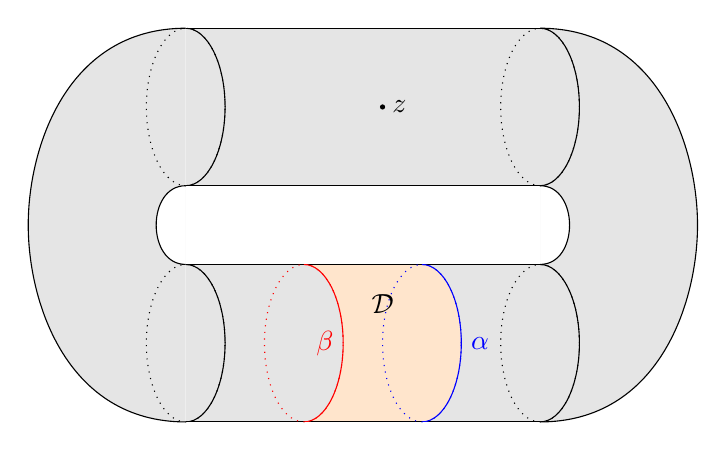
\begin{tikzpicture}



    \begin{scope}[]
    \begin{scope}[]
    
    \draw[fill=gray!20] (-2,-1.5) .. controls (-3.5,-1.5) and (-4,0) .. (-4,1) .. controls (-4,2) and (-3.5,3.5) .. (-2,3.5) (-2,1.5) .. controls (-2.5,1.5) and (-2.5,0.5) .. (-2,0.5);
    
    \end{scope}
    
    
    
    \begin{scope}[xscale=-1, shift={(-0.5,0)}]]
    
    \draw[fill=gray!20] (-2,-1.5) .. controls (-3.5,-1.5) and (-4,0) .. (-4,1) .. controls (-4,2) and (-3.5,3.5) .. (-2,3.5) (-2,1.5) .. controls (-2.5,1.5) and (-2.5,0.5) .. (-2,0.5);
    
    \end{scope}
    \fill[gray!20]  (-2,0.5) rectangle (2.5,-1.5);
    \fill[gray!20]  (-2,3.5) rectangle (2.5,1.5);

    \end{scope}
    
    \begin{scope}[]
    
    \fill[orange!20]  (1,-0.5) ellipse (0.5 and 1);
    \fill[orange!20]  (-0.5,0.5) rectangle (1,-1.5);
    \fill[gray!20]  (-0.5,-0.5) ellipse (0.5 and 1);
    \end{scope}
        \draw (-2,-1.5) -- (2.5,-1.5) (-2,0.5) -- (2.5,0.5) (-2,1.5) -- (2.5,1.5) (-2,3.5) -- (2.5,3.5);
    
    
    \begin{scope}[]
    
    \draw[dotted]  (-2,-0.5) ellipse (0.5 and 1);
    \clip  (-2,0.5) rectangle (-1,-1.5);
    \draw  (-2,-0.5) ellipse (0.5 and 1);
    \end{scope}
    
    
    
    \begin{scope}[red, shift={(1.5,0)}]
    
    \draw[dotted]  (-2,-0.5) ellipse (0.5 and 1);
    \clip  (-2,0.5) rectangle (-1,-1.5);
    \draw  (-2,-0.5) ellipse (0.5 and 1);
    \end{scope}
    
    
    \begin{scope}[blue, shift={(3,0)}]
    
    \draw[dotted]  (-2,-0.5) ellipse (0.5 and 1);
    \clip  (-2,0.5) rectangle (-0.5,-1.5);
    \draw  (-2,-0.5) ellipse (0.5 and 1);
    \end{scope}
    
    \begin{scope}[shift={(4.5,0)}]
    
    \draw[dotted]  (-2,-0.5) ellipse (0.5 and 1);
    \clip  (-2,0.5) rectangle (-1,-1.5);
    \draw  (-2,-0.5) ellipse (0.5 and 1);
    \end{scope}
    
    \begin{scope}[shift={(4.5,3)}]
    
    \draw[dotted]  (-2,-0.5) ellipse (0.5 and 1);
    \clip  (-2,0.5) rectangle (-1,-1.5);
    \draw  (-2,-0.5) ellipse (0.5 and 1);
    \end{scope}
    
    \begin{scope}[shift={(0,3)}]
    
    \draw[dotted]  (-2,-0.5) ellipse (0.5 and 1);
    \clip  (-2,0.5) rectangle (-1,-1.5);
    \draw  (-2,-0.5) ellipse (0.5 and 1);
    \end{scope}
    
    
    
    \node[left, red] at (0,-0.5) {$\beta$};
    \node[right, blue] at (1.5,-0.5) {$\alpha$};
    \node at (0.5,0) {$\mathcal D$};
    
    \node[circle, fill=black, scale=.2] at (0.5,2.5) {};
    \node[right] at (0.5,2.5) {$z$};
    
    \end{tikzpicture}
    If the diagram is chosen so that $\alpha, \beta$ are disjoint, then the Lagrangian intersection Floer cohomology $\HF(\alpha, \beta)$ vanishes.
    %label:"fig:admissibleHeegaardDiagram"
%author:JeffHicks
%name:"admissible HeegaardDiagram"
%type:"figure"
%parent:def:weaklyAdmissibleHeegaardDiagram
%caption:"An admissible Heegaard diagram"


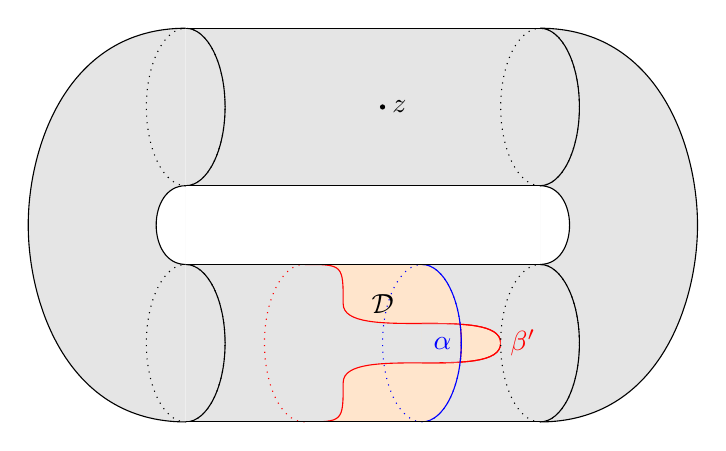
\begin{tikzpicture}

    \begin{scope}[]
    \begin{scope}[]
    
    \draw[fill=gray!20] (-2,-1.5) .. controls (-3.5,-1.5) and (-4,0) .. (-4,1) .. controls (-4,2) and (-3.5,3.5) .. (-2,3.5) (-2,1.5) .. controls (-2.5,1.5) and (-2.5,0.5) .. (-2,0.5);
    
    \end{scope}
    
    
    
    \begin{scope}[xscale=-1, shift={(-0.5,0)}]]
    
    \draw[fill=gray!20] (-2,-1.5) .. controls (-3.5,-1.5) and (-4,0) .. (-4,1) .. controls (-4,2) and (-3.5,3.5) .. (-2,3.5) (-2,1.5) .. controls (-2.5,1.5) and (-2.5,0.5) .. (-2,0.5);
    
    \end{scope}
    \fill[gray!20]  (-2,0.5) rectangle (2.5,-1.5);
    \fill[gray!20]  (-2,3.5) rectangle (2.5,1.5);
    
    \end{scope}
    
    \begin{scope}[]
    
    \fill[orange!20]  (1,-0.5) ellipse (0.5 and 1);
    \fill[orange!20]  (-0.5,0.5) rectangle (1,-1.5);
    \fill[gray!20]  (-0.5,-0.5) ellipse (0.5 and 1);
    \end{scope}
    
    
    \begin{scope}[]
    
    \draw[dotted]  (-2,-0.5) ellipse (0.5 and 1);
    \clip  (-2,0.5) rectangle (-1,-1.5);
    \draw  (-2,-0.5) ellipse (0.5 and 1);
    \end{scope}
    
    
    
    \begin{scope}[red, shift={(1.5,0)}]
    
    \draw[dotted]  (-2,-0.5) ellipse (0.5 and 1);
    \clip  (-2,0.5) rectangle (0.5,-1.5);
    \draw[fill=gray!20] (-2,0.5) .. controls (-1.5,0.5) and (-1.5,0.5) .. (-1.5,0) .. controls (-1.5,-0.5) and (0.5,0) .. (0.5,-0.5) .. controls (0.5,-1) and (-1.5,-0.5) .. (-1.5,-1) .. controls (-1.5,-1.5) and (-1.5,-1.5) .. (-2,-1.5);
    
    \clip  (-0.5,0) rectangle (0.5,-1);
    \draw[fill=orange!20] (-1.5,0) .. controls (-1.5,-0.5) and (0.5,0) .. (0.5,-0.5) .. controls (0.5,-1) and (-1.5,-0.5) .. (-1.5,-1);
    \clip (-1.5,0) .. controls (-1.5,-0.5) and (0.5,0) .. (0.5,-0.5) .. controls (0.5,-1) and (-1.5,-0.5) .. (-1.5,-1);
    
    \draw[fill=gray!20]  (-0.5,-0.5) ellipse (0.5 and 1);
    \draw (-1.5,0) .. controls (-1.5,-0.5) and (0.5,0) .. (0.5,-0.5) .. controls (0.5,-1) and (-1.5,-0.5) .. (-1.5,-1);
    
    \end{scope}
    
    
    \begin{scope}[blue, shift={(3,0)}]
    
    \draw[dotted]  (-2,-0.5) ellipse (0.5 and 1);
    \clip  (-2,0.5) rectangle (-0.5,-1.5);
    \draw  (-2,-0.5) ellipse (0.5 and 1);
    \end{scope}
    
    \begin{scope}[shift={(4.5,0)}]
    
    \draw[dotted]  (-2,-0.5) ellipse (0.5 and 1);
    \clip  (-2,0.5) rectangle (-1,-1.5);
    \draw  (-2,-0.5) ellipse (0.5 and 1);
    \end{scope}
    
    \begin{scope}[shift={(4.5,3)}]
    
    \draw[dotted]  (-2,-0.5) ellipse (0.5 and 1);
    \clip  (-2,0.5) rectangle (-1,-1.5);
    \draw  (-2,-0.5) ellipse (0.5 and 1);
    \end{scope}
    
    \begin{scope}[shift={(0,3)}]
    
    \draw[dotted]  (-2,-0.5) ellipse (0.5 and 1);
    \clip  (-2,0.5) rectangle (-1,-1.5);
    \draw  (-2,-0.5) ellipse (0.5 and 1);
    \end{scope}
    
    
    
    \node[right, red] at (2,-0.5) {$\beta'$};
    \node[left, blue] at (1.5,-0.5) {$\alpha$};
    \node at (0.5,0) {$\mathcal D$};
    
    \node[circle, fill=black, scale=.2] at (0.5,2.5) {};
    \node[right] at (0.5,2.5) {$z$};
    
    \draw (-2,-1.5) -- (2.5,-1.5) (-2,0.5) -- (2.5,0.5) (-2,1.5) -- (2.5,1.5) (-2,3.5) -- (2.5,3.5);
    
\end{tikzpicture}
    However, if the diagram is chosen so that $\alpha, \beta'$ intersect transversely, the Lagrangian intersection Floer cohomology (with $\ZZ/2\ZZ$ coefficients) is $\ZZ/2\ZZ\oplus \ZZ/2\ZZ$. Note that $\beta'$ can be chosen so that it is Hamiltonian isotopic to $\beta$.
    
    The discrepancy between these two answers comes from the non-convergence of the homotopy between the composition of continuation maps  $f\circ g:\CF(\alpha, \beta')\to \CF(\alpha, \beta) \to \CF(\alpha, \beta')$ and $\id: \CF(\alpha, \beta')$ over $\ZZ/2\ZZ$ coefficients. The presence of an annulus between $\alpha, \beta$ is the culprit for the non-convergence.

    If one instead chooses to use Novikov (instead of $\ZZ/2\ZZ$ coefficients) one can obtain a 

    To rule out this phenomenon, we only look at strips which avoid the marked point $z$, and will impose a criterion (admissible Heegaard diagrams) which will, in this setting, preclude the existence of annuli disjoint from the marked point $z$.  In general, the admissibility criterion will limit us to configurations of cycles for which the number of holomorphic strips contributing to the Floer differential is finite.


